\documentclass[bachelor]{SCWorks}
% Тип обучения (одно из значений):
%    bachelor   - бакалавриат (по умолчанию)
%    spec       - специальность
%    master     - магистратура
% Форма обучения (одно из значений):
%    och        - очное (по умолчанию)
%    zaoch      - заочное
% Тип работы (одно из значений):
%    coursework - курсовая работа (по умолчанию)
%    referat    - реферат
%  * otchet     - универсальный отчет
%  * nirjournal - журнал НИР
%  * digital    - итоговая работа для цифровой кафдры
%    diploma    - дипломная работа
%    pract      - отчет о научно-исследовательской работе
%    autoref    - автореферат выпускной работы
%    assignment - задание на выпускную квалификационную работу
%    review     - отзыв руководителя
%    critique   - рецензия на выпускную работу
% Включение шрифта
%    times      - включение шрифта Times New Roman (если установлен)
%                 по умолчанию выключен
\usepackage{preamble}

\begin{document}

% Кафедра (в родительном падеже)
\chair{математической кибернетики и компьютерных наук}

% Тема работы
\title{Генеративное компьютерное зрение}

% Курс
\course{2}

% Группа
\group{211}

% Факультет (в родительном падеже) (по умолчанию "факультета КНиИТ")
% \department{факультета КНиИТ}

% Специальность/направление код - наименование
\napravlenie{02.03.02 "--- Фундаментальная информатика и информационные технологии}
% \napravlenie{02.03.01 "--- Математическое обеспечение и администрирование информационных систем}
% \napravlenie{09.03.01 "--- Информатика и вычислительная техника}
%\napravlenie{09.03.04 "--- Программная инженерия}
% \napravlenie{10.05.01 "--- Компьютерная безопасность}

% Для студентки. Для работы студента следующая команда не нужна.
% \studenttitle{Студентки}

% Фамилия, имя, отчество в родительном падеже
\author{Пицика Харитона Николаевича}

% Заведующий кафедрой 
\chtitle{доцент, к.\,ф.-м.\,н.}
\chname{С.\,В.\,Миронов}


% Руководитель ДПП ПП для цифровой кафедры (перекрывает заведующего кафедры)
% \chpretitle{
%     заведующий кафедрой математических основ информатики и олимпиадного\\
%     программирования на базе МАОУ <<Ф"=Т лицей №1>>
% }
% \chtitle{г. Саратов, к.\,ф.-м.\,н., доцент}
% \chname{Кондратова\, Ю.\,Н.}

% Научный руководитель (для реферата преподаватель проверяющий работу)
\satitle{доцент}
\saname{Б.\,А.\,Филиппов}

% Руководитель практики от организации (руководитель для цифровой кафедры)


% Руководитель НИР
%\nirtitle{доцент, к.\,п.\,н.} % степень, звание
%\nirname{М.\,И.\,Сафрончик}

% Семестр (только для практики, для остальных типов работ не используется)
%\term{}

% Наименование практики (только для практики, для остальных типов работ не
% используется)
%\practtype{учебная}

% Продолжительность практики (количество недель) (только для практики, для
% остальных типов работ не используется)
%\duration{2}

% Даты начала и окончания практики (только для практики, для остальных типов
% работ не используется)
%\practStart{01.07.2022}
%\practFinish{13.01.2023}

% Год выполнения отчета
\date{2025}

\maketitle

% Включение нумерации рисунков, формул и таблиц по разделам (по умолчанию -
% нумерация сквозная) (допускается оба вида нумерации)
\secNumbering
\tableofcontents

\intro
Генеративное компьютерное зрение является областью глубокого обучения, которая фокусируется на генерации новых изображений, опираясь на исходный набор данных и меток. Компьютерное зрение находит применение во множестве областей, в том числе и в электронной коммерции, развлечении и дизайне. В наше время существует большое количество моделей, способных генерировать изображения. В зависимости от доступных ресурсов, исходного набора данных и желаемых результатов, среди моделей и архитектур выбирается наиболее подходящая. 

В последнее время наблюдается резкий рост популярности интернет"=магазинов одежды. Несмотря на это, большинство покупаталей всё ещё обеспокоено тем, как заказываемый товар будет сидеть на человеке в зависимости от телосложения, позы и других факторов. Исходя из этого, возможность виртуальной примерки одежды является востребованной задачей, решение которой позволит покупателям сэкономить время и денеждные средства, а также улучшит впечатление от дальнейших покупок.

Классическая задача виртуальной примерочной включает в себя генерацию реалистичного изображения человека в выбранной одежде, используя только 2D"=фотографии пользователя или товара. Главные вызовы включают в себя сохранение индивидуальных особенностей человека на фото, корректная деформация и наложение новой одежды на фото с учётом позы и угла, борьба с артефактами и потерей важных признаков фотографии. Внедрение систем виртуальных примерочных позволяет автоматизировать процесс подбора одежды, а также расширить доступность моды в мире. 

В рамках данной работы проведён анализ 3 наиболее популярных и передовых подходов к решению задачи виртуальной примерочной (\texttt{VITON}, \texttt{Virtual Try-On}): \texttt{LaDI"=VITON}, \texttt{PASTA"=GAN++} и \texttt{PromptDresser}. \texttt{LaDI"=VITON} фокусируется на реалистичности итоговой фотографии, \texttt{PASTA"=GAN++} использует продвинутые механизмы фрагментации и наложения одежды, а \texttt{PromptDresser} в свою очередь позволяет манипулировать процессом с помощью интегрированной системы обработки текстовых запросов.  Для объективного сравнения в рамках данной работы будет вручную составлен набор данных, а также по результатам моделей с помощью метрик будет установлено, в каких ситуациях какой подход оказывается лучше.


\section{Теоретическая часть}
\subsection{Основные понятия компьютерного зрения}
Компьютерное зрение "--- область искуственного интеллекта, которая занимается разработкой и оптимизацией технологий для обработки визуальной информации из изображений и видео. Основная суть комьютерного зрения "--- получение более структурированной информации, пригодной для дальнейшего использования в приложениях \cite{cv_intro}.

Среди процессов решения задачи компьютерного зрения можно выделить:
\begin{itemize}
    \item Сбор визуальных данных "--- получение исходного набора данных для дальнейшего обучения модели;
    \item Предобработка данных "--- подготовка данных для модели: изменение размера, нормализация яркости, обрезка ненужной информации;
    \item Интерпретация "--- применение алгоритмов классического машинного обучения и глубокого обучения для решения определённой задачи. Например, решение задачи классификации или сегментации. 
\end{itemize}

Глубокое обучение является одним из ключевых направлений машинного обучения. Решения из глубокого обучения предполагают использование многослойных искусственных нейронных сетей для автоматического извлечения признаков для дальнейшей классификации или распознавания. 

Генеративные модели представляют собой класс алгоритмов, конечной целью которых является аппроксимация распределения исходного набора данных для дальнейшего синтеза данных. В контексте компьютерного зрения, генеративные модели применяются для генерации новых, фотореалистичных изображений. Именно эти модели применяются для решения задачи виртуальной примерочной, поскольку необходимо сгенерировать новое изображение исходной модели с другой одеждой. К генеративным моделям относят порождающие состязательные сети, диффузионные модели, а также вариацонные автокодировщики \cite{generative_plus_gan}.
\subsection{Порождающие состязательные сети}
Порождающие состязательные сети (\texttt{Generative Adversarial Network}, \texttt{GAN}) "--- модель, предназначенная для генерации качественных изображений на основе существующего набора данных. Впервые была предложена в 2014 году в деятельности Иэна Гудфеллоу. Классическая реализация порождающих состязательных сетей состоит из двух искусственных нейронных сетей, цель которых "--- <<одолеть>> друг друга.

Одна из нейронных сетей в \texttt{GAN} называется генератором (generator) и предназначена для порождения объектов в пространстве данных, а вторая нейронная сеть является дискриминатором (discriminator). Задача дискриминатора заключается в классификации подаваемых на вход изображений, в том числе порожденных вышеописанным генератором. Таким образом, задача дискриминатора сводится к успешной классификации, а задача генератора "--- минимизировать оценивающую функцию дискриминатора \cite{gan_intro}.

Поскольку нейронные сети сами по себе не умеют генерировать новые примеры из ничего, необходимо, чтобы модели преобразовывали случайны входы из стандартного нормального распределения $\mathcal{N}(0, 1)$. Таким образом, нейронная сеть будет преобразовывать распределение $\mathcal{N}(0, 1)$ в распределение данных. Формально, генератор можно записать следующим образом:


\begin{equation}
    G = G(z; \theta_g): Z \rightarrow X,
\end{equation}
где $Z$ "--- пространство латентных факторов, где есть распределение $p_z(z)$. 

Дискриминатор выглядит следующим образом:
\begin{equation}
    D = D(x; \theta_d): X \rightarrow [0, 1]
\end{equation}
В данном случае, данные конвертируется в отрезок $[0, 1]$, который означает вероятность того, что поданный на вход пример не является выходом генератора. Таким образом, дискриминатор хочет максимизировать следующую величину:
\begin{equation}
    \mathbb{E}_{x \sim p_{data}(x)}[\log D(x)] + \mathbb{E}_{x \sim p_{gen}(x)}[1 - \log D(x)],
\end{equation}
где $p_{gen}(x)$ "--- элемент из порождаемого генератором распределения ,$p_{gen}(x) = G_{z \sim p_z}(x)$

В общем случае, генеративные состязательные сети решают задачу оптимизации, широко известную как <<задача minimax>>: \cite{nikolenko_dl}
\begin{equation}
    \min\limits_{G}\max\limits_{D}V(D, G),
\end{equation}
где
\begin{equation}
    V(D, G) = \mathbb{E}_{x \sim p_{gen}(x)}[\log D(x)] + \mathbb{E}_{z \sim p_{z}(z)}[1 - \log D(G(z))]
\end{equation}

Общий вид порождающих состязательных сетей (\texttt{pipeline}) можно рассмотреть на рисунке \ref{fig:gan_overview}\cite{gan_intro}.

\begin{figure}[H]
    \centering
    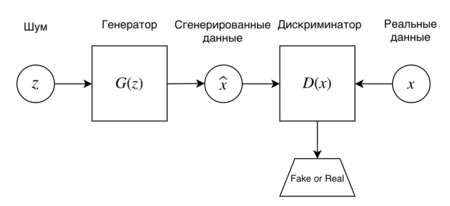
\includegraphics[width=0.7\linewidth]{images/gan_overview.png}
    \caption{Классическая реализация GAN}
    \label{fig:gan_overview}
\end{figure}

Общий процесс обучения модели относительно распределений данных можно увидеть на рисунке \ref{fig:gan_train} \cite{gan_intro}.
\begin{figure}[H]
    \centering
    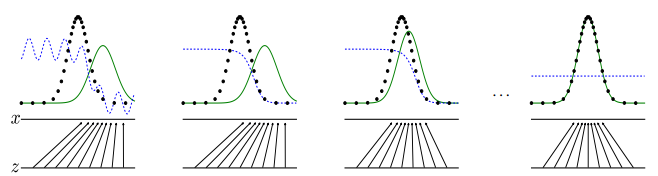
\includegraphics[width=0.9\linewidth]{images/gan_train.png}
    \caption{Процесс обучения: синяя пунктирная линия "--- дискриминантное распределение, чёрная пунктирная линия "--- порождающее распределение, зеленая сплошная линия "--- генеративное распределение, верхняя горизонтальная линия "--- часть области из $\mathbb{X}$, нижняя горизонтальная линия "--- область, из которой отбирается выборка $z$.}
    \label{fig:gan_train}
\end{figure}

Одним из недостатков архитектуры \texttt{GAN} является вероятное схлопывание в моду (mode collapse), когда генератор находит распределение, данные из которого дискриминатор не может корректно классифицировать. В этом случае существует вероятность, что генератор остановится в этом распределении и продолжит генерировать изображения, опираясь только на эту часть признакового пространства \cite{gan_intro}.

\subsubsection{Использование \texttt{GAN}}
При обучении, модели могут использовать парные и непарные изображения. В зависимости от этого параметра, задача ставится по"=разному. Для парных данных задача является обучением с учителем (supervised learning), поскольку у модели есть чёткое обозначение, на какую картинку по пикселям стоит ориентироваться. В то время как непарные данные являются обучением без учителя (unsupervised learning), то есть не существует чёткого обозначения, во что должно превратиться исходное изображение. С точки зрения качества изображения это может повлиять, однако вариант с задачей без учителя является более приблежённым к реальной жизни и именно на непарных данных обучаются модели для коммерческих целей \cite{unpaired}.

Рассмотрим применение порождающих состязательных сетей в коммерческой разработке. В рамках анализа было рассмотренно решение \texttt{PASTA"=GAN++}, использующее непарные изображения для обучения. Пусть $I_s$ "--- исходное изображение, модель на котором одета в бельё $G_s$. Задача виртуальной примерочной "--- сгенерировать изображение $I'_t$, являющееся копией изображения $I_t$ в одежде $G_s$. Для достижения данного результата, \texttt{PASTA"=GAN++} использует модуль распутывания с маршрутизацией патчей, результат работы которого можно увидеть на изображении \ref{fig:gan_prdm} \cite{pasta_gan}.
\begin{figure}[H]
    \centering
    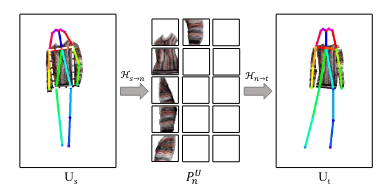
\includegraphics[width=0.6\linewidth]{images/gan_prdm_res.png}
    \caption{Модуль распутывания с маршрутизацией патчей}
    \label{fig:gan_prdm}
\end{figure}

Одежда $G_s$ преобразуется в патчи $P_n$, которые в свою очередь деформируются для перехода к деформированной одежде $G_t$. Таким образом, данный модуль делает некоторое предсказание позы человека, основываясь на нормализованных патчах. $G_t$ соответствует позе целевого человека.

Затем для генерации реалистичного результата примерки одежды, применяется модуль \texttt{StyleGAN2}, где происходит синтезация парсинга человека $S_t$. Данный парсинг отображает основные детали, такие как поза и одежда, чтобы на основе особенностей накладываемой одежды сделать нужные искажения.

Затем применяется модуль \texttt{Spatially-Adaptive Residual Module}, который встраивается в генератор \texttt{GAN} и который отвечает за наложение искажённой одежды на новую позу. Этот модуль использует метод inpainting и SPADE"=нормализацию для модуляции и визуализации полученных признаков \cite{pasta_gan} \cite{spade}.

При обучении \texttt{PASTA"=GAN++} в качестве функций потерь были использованы:
\begin{equation}
    L_{rec} = \sum_{I \in{\tilde{I'}, I'}}||I - I_s||_1;
\end{equation}

\begin{equation}
    L_{perc} = \sum_{I \in{\tilde{I'}, I'}}\sum_{k=1}^5 \lambda_k||\phi_k(I) - \phi_k(I_s)||_1.
\end{equation}
$L_{rec}$ является разницей между признаками исходного изображения и признаками изображения, которое удалось сгенерировать на его основе. $L_{perc}$ предназначен для фиксации перцепционных различий между изображениями, таких как несоответствие содержания и стиля, которые не всегда очевидны на уровне пикселей \cite{pasta_gan}.

В рамках данного анализа было рассмотрено именно это решение, поскольку \texttt{PASTA"=GAN++} является первым переходом от парных изображений в сфере порождающих состязательных сетей, а также является универсальным решением для любой части туловища: генерировать можно как и верхнюю, так и нижнюю одежды.
\subsection{Диффузионные нейронные сети}
Диффузионным нейронным сетям удалось оказать заметное влияние на сферу обработки картинок и видеорядов. Диффузионные нейронные сети являются подкатегорией глубоких генеративных моделей. Они состоят из этапов прямой и обратной диффузий и генерируют новые данные, аналогичные тем, на которых они обучались. В отличие от традиционных генеративных моделей, таких как GAN и вариационные автокодировщики (\texttt{VAE}), диффузионные модели реализуют процесс поэтапного преобразования шума в осмысленные данные, что обеспечивает высокое качество синтезируемых изображений и стабильность обучения \cite{diffusion_intro}.

Подход диффузионных нейронных сетей обусловлен неравновесной термодинамикой: модели плавно накладывают шум на объект из тренировочной выборки, а затем обучаются обращать процесс диффузии \cite{diffusion_thermo}. Целью этого процесса является получение осмысленных изображений, имеющих сходство с исходным набором данных. В отличие от \texttt{VAE}, где латентное пространство ограничено и требуется оптимизация вариационной нижней оценки, диффузионные модели используют фиксированную процедуру зашумления и обладают латентным пространством высокой размерности, что способствует более гибкой генерации.

Процесс зашумления исходного распределения осуществляется с помощью планировщика шума, который указывает, в каких пропорциях необходимо добавлять шум. Регулировать это можно с помощью параметра $t$: чем больше этот параметр, тем больше шума будет добавлено:
\begin{gather}
z_{x, t = 0} = x\\ \label{math:dnn1}
z_{x, t = T} \sim \mathcal{N}(0, I), ~~ \text{где I - некоторая величина.}
\end{gather}
Генерация изображения начинается с выбора начального вектора из стандартного нормального распределения $\mathcal{N}(0, 1)$, после чего модель $D_{\theta}$ итеративно очищает вектор от шума, приближая его к целевому изображению.

Процесс очистки изображения от Гауссовского шума задаётся следующей функцией потерь:
\begin{equation}
    L(x, c, t) = ||D_{\theta}(z_{x, t}, c) - x||_2^2,
\end{equation}
где $x$ "--- исходное изображение, $c$ - дополнительные условия (например, текстовая разметка).

В упрощённом виде, работу диффузионных нейронных сетей можно увидеть на рисунке \ref{fig:dnn_example}.
\begin{figure}[H]
    \centering
    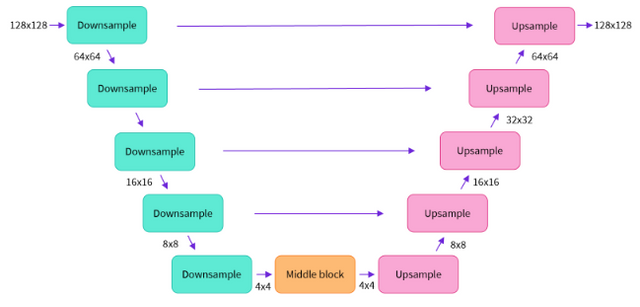
\includegraphics[width=0.8\linewidth]{images/dnn_example.png}
    \caption{Диффузионная нейронная сеть}
    \label{fig:dnn_example}
\end{figure}

Диффузионные модели демонстрируют высокое качество синтезированных изображений, зачастую превосходящие своих конкруентов в детализации и реалистичности. Помимо этого, процесс обучения является стабильным, поскольку происходят неизменяющиеся действия в рамках каждой отдельной генерации. К недостаткам модели можно отнести высокую требовательность к вычислительной машине, поскольку для каждой генерации требуется сделать большое количество операций итеративного очищения вектора от шума, что в теории может затруднить интеграцию модели для работы в реальном времени. Качество сгенерированных результатов сильно зависит от настройки планировщика шума. Таким образом, неправильно подобранные параметры планировщика шума могут сильно исказить результаты.

\subsubsection{Применение \texttt{DNN}}
Выбор именно \texttt{LaDI"=VITON} обоснован тем, что данное решение впервые предлагает подход через латентные диффузионные модели (\texttt{Latent Diffusion Models, LDM}). \texttt{LDM} включают в себя автокодировщик $\mathcal{A}$ с кодировщиком $\mathcal{E}$ и декодировщиком $\mathcal{D}$, модель \texttt{U"=Net}  деноизации текста с временными условиями $\epsilon_{\theta}$, а также кодировщик текста \texttt{CLIP} $T_E$, который принимает на вход $Y$. Обучение $\epsilon_{\theta}$ осуществляется через следующую функцию потерь:
\begin{gather}
    L = \mathbb{E}_{\mathcal{E}(I),Y, \epsilon \sim \mathcal{N}(0, 1), t}[||\epsilon - \epsilon_{\theta}(\phi, \psi)||_2^2],
\end{gather}
где $t$ представляет собой шаг диффузии, $\phi = z_t$, $z_t$ "--- закодированное изображение $\mathcal{E}(I)$, в котором был добавлен шум $\mathcal{N}(0, 1)$, и $\psi = [t, T_E(Y)]$.
Целью данного процесса является генерация нового изображения $\tilde{I}$ из исходного изображения $I$, сочетающее в себе $I$ и одежду, предоставленную пользователем. Общий вид модели можно увидеть на рисунке \ref{fig:ladi_pipeline} \cite{ladi}.
\begin{figure}[H]
    \centering
    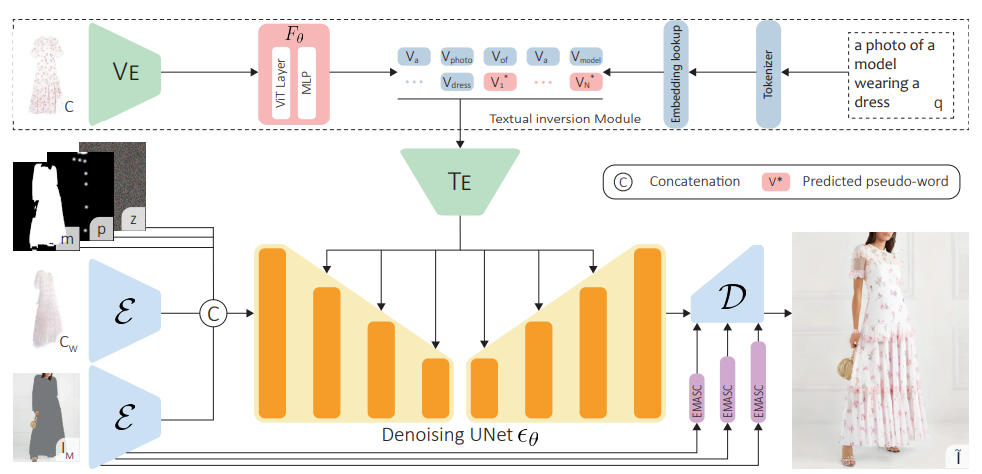
\includegraphics[width=0.94\linewidth]{images/ladi_pipeline.png}
    \caption{Общий вид \texttt{LADI"=VITON}}
    \label{fig:ladi_pipeline}
\end{figure}

Использование латентных диффузионных моделей позволяет работать в сжатом латентном пространстве, что снижает вычислительные затраты и повышает качество синтеза по сравнению с генерацией непосредственно в пиксельном пространстве. Текстовая инверсия с помощью \texttt{CLIP}-кодировщика эффективно кодирует визуальные характеристики одежды в условное пространство, обеспечивая точное управление процессом генерации и сохранение текстурных деталей. Модель \texttt{U-Net} с временными условиями обучается предсказывать шум на каждом шаге диффузии, что обеспечивает постепенное и стабильное восстановление изображения с учётом заданных условий. Дополнительные механизмы, такие как \texttt{Enhanced Mask-Aware Skip Connection} (\texttt{EMASC}), улучшают сохранение высокочастотных деталей и снижают ошибки реконструкции, что особенно важно для реалистичного отображения мелких деталей одежды. Обзор \texttt{EMASC} можно увидеть на рисунке \ref{fig:ladi_emasc} \cite{ladi}.
\begin{figure}[H]
    \centering
    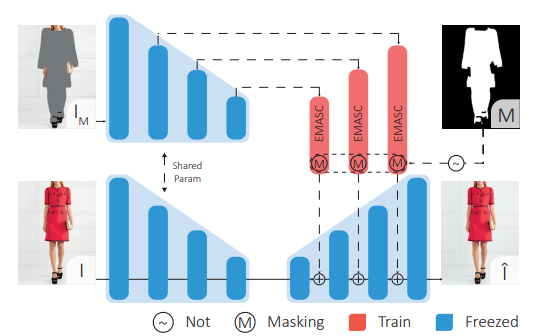
\includegraphics[width=0.9\linewidth]{images/ladi_emasc.png}
    \caption{Общий вид \texttt{EMASC}}
    \label{fig:ladi_emasc}
\end{figure}

Формально, модуль \texttt{EMASC} можно записать следующим образом:
\begin{gather}
    EMASC_i = f(E_i) * NOT(m_i) \\
    D_i = D_{i-1} + EMASC_i,
\end{gather}
где $f$ "--- обученная нелинейная функция, $E_i$ это $i$"=я карта признаков из кодировщика $\mathcal{E}$, $D_i$ есть соответствующая карта признаков из декодировщика, а $m_i$ получается в результате изменения размера маски $M$ в соответствии с пространственным измерением $E_i$.

Итоговая функция потерь имеет следующий вид:
\begin{gather}
    L = \mathbb{E}_{\mathcal{E}(I), \widehat{Y}, \epsilon \sim \mathcal{N}(0, 1),t,\mathcal{E}(I_M), M, p, \mathcal{E}(C_W)}[||\epsilon - \epsilon_{\theta}(\phi, \psi)||_2^2],
\end{gather}
где $\psi = [t;T_E(\widehat{Y})]$.
\subsection{Большие мультимодальные модели}
Большие мультимодальные модели (\texttt{Large Multimodal Model}, \texttt{LMM}) способны обрабатывать разные входные данные, например видео, аудио, изображение. Способность обрабатывать информацию из разных данных делают эту модель некоторым расширением возможностей классических языковых моделей (\texttt{LLM}). В общем смысле, \texttt{LMM} представляют собой комбинацию \texttt{LLM} и унифицированных под каждый тип данных энкодеров, например свёрточные нейронные сети для изображений, трансформеры для текстов, спектрограммы для аудио. Затем происходит операция связывания (\texttt{fusion}), что обеспечивает взаимодействие между признаками разных модальностей, а также даёт возможность составлять комбинированные функции потерь.

В контексте курсовой работы, \texttt{LMM} применяется для генерации подробных и структурированных описаний одежды и позы человека на входном изображении, которые в дальнейшем можно использовать, например, в латентных диффузионных моделях (\texttt{Latent Diffusion Model}, \texttt{LDM}). Операция применения выходов одной модели для запуска другой модели называется стэкинг (\texttt{stacking}). После перечисления аттрибутов позы и одежды, выбираются $n^{\{p, c\}}$ наиболее информативных признаков: $A^{\{p, c\}} = \{a_1^{\{p, c\}}, \dots, a_{n^{\{p, c\}}}^{\{p, c\}}\}$. В зависимости от условий, можно контроллировать процесс отбора признаков. Так, в силу ограниченности длины лексем в кодировщике \texttt{CLIP}, стоит выбирать более глобальные признаки, такие как материал, цвет. Используя описания вместо \texttt{DensePose}, удаётся сохранить архитектуру \texttt{text"=to"=image} \cite{promptdresser}.

При входном изображении $x \in \{x^p, x^c\}$ и \texttt{LMM} $\mathcal{M}$, предсказанные описания $\mathcal{K}^{\{p, c\}}$ можно получить следующим образом:
\begin{gather}
    \mathcal{K}^{\{p, c\}} = \{k_1^{\{p, c\}}, \dots, k_{n^{\{p, c\}}}^{\{p, c\}}\} = \mathcal{M}(x|\mathcal{P}, \mathcal{D}_{ex}^{\{p, c\}}, \mathcal{T}^{\{p, c\}}),
\end{gather}
где $\mathcal{P}$ есть входной промпт, $\mathcal{D}_{ex}^{\{p, c\}}$ "--- набор данных для обучения в контексте, и $\mathcal{T}^{\{p, c\}}$ "--- описание задачи. Процесс генерации маски на основе текстового запроса можно увидеть на изображении \ref{fig:lmm_maskgener} \cite{promptdresser}.

\begin{figure}[H]
    \centering
    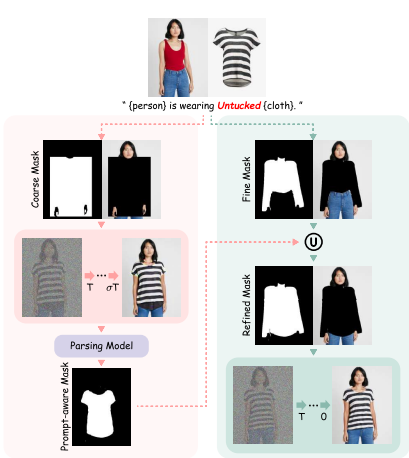
\includegraphics[width=0.75\linewidth]{images/lmm_maskgener.png}
    \caption{Процесс генерации маски с помощью \texttt{LMM}}
    \label{fig:lmm_maskgener}
\end{figure}

Основным преимуществом \texttt{LMM} является универсальность, поскольку модель может работать с несколькими модальностями. Помимо этого, для задач виртуальной примерочной полезно связывать изображение с его текстовым описанием, с чем мультимодальная модель очень хорошо справляется, а обучение на разнотипных данных даёт устойчивость к качеству исходных изображений, что позволяет генерировать более стабильные результаты. К недостаткам данной модели можно отнести факт того, что без тщательной фильтрации \texttt{LMM} может включать в промпты упоминания старой одежды, что приводит к артефактам и некорректному редактированию изображения. Помимо этого, точность и полнота промптов зависит от выбранной \texttt{LMM} (\texttt{GPT"=4o}, \texttt{LLaVA} и др.), что может привести к нестабильным результатом при смене модели. Помимо этого, мультимодальная модель может не так точно передавать более мелкие признаки, такие как узор одежды, крой, материал, что может снизить итоговое качество.

\subsubsection{Использование \texttt{LMM}}
Метод \texttt{PromptDresser} ориентируется на создание виртуальной примерочной, которая будет регулироваться посредством текстовых запросов. Так, задача сводится к генерации изображения $x^p$ на основе изображения $x^c$ с помощью методов обработки текста, предоставляемых в \texttt{LMM}. Общий подход к решению данной задачи можно рассмотреть на изображении \ref{fig:prompt_pipeline} \cite{promptdresser}.

Подход \texttt{PromptDresser} основывается на \texttt{LDM}, который состоит из трёх основных компонент: \texttt{VAE} с кодировщиком $\mathcal{E}(\cdot)$ и декодировщиком $\mathcal{G}(\cdot)$, текстовый кодировщик $\tau(\cdot)$ и основная \texttt{UNet} $\epsilon_0$. Предобученный \texttt{VAE} кодирует исходное изображение $x$ в в латентное пространство меньшей размерности: $z_0 = \mathcal{E}(x)$. Затем происходит восстановление в $\texttt{RGB}$ посредством декодировщика: $\hat{x} = \mathcal{G}(z_0)$. \texttt{UNet} предобучена для предсказания значения $z_0$ на основе $z_t$, где 
\begin{gather}
    z_t = \mathcal{N}(z_t; \sqrt{\overline{\alpha}}z_0, (1 - \overline{\alpha_t})I)
\end{gather}
Функция потерь \texttt{LDM} выглядит следующим образом:
\begin{gather}
    \mathcal{L}_{LDM} = \mathbb{E}_{z_0 \sim \mathcal{E}(x), \epsilon \sim \mathcal{N}(0, I), y, t}[||\epsilon - \epsilon_0 (z_t, t, \tau(y)||_2^2]
\end{gather}
Данная функция нацелена на уменьшение разницы между получившимся шумом $\epsilon$, и шумом, предсказанным с помощью \texttt{UNet}.
\begin{figure}[H]
    \centering
    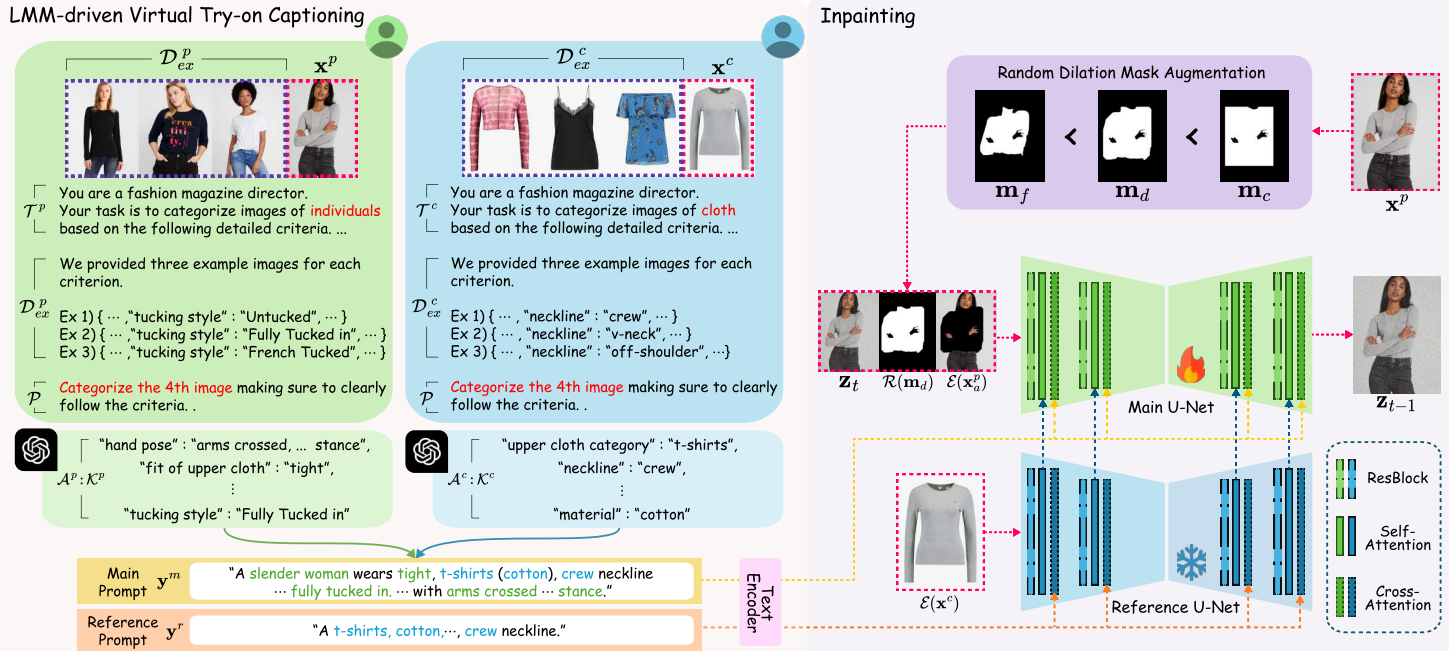
\includegraphics[width=0.95\linewidth]{images/prompt_pipeline.png}
    \caption{Подход \texttt{PromptDresser} в решении задачи \texttt{VITON}}
    \label{fig:prompt_pipeline}
\end{figure}
Далее, с помощью \texttt{GPT"=4o} происходит генерация текстовых подсказок, что позволяет разделить описание позы и описание одежды. Вводится метод генерации масок от грубых (\texttt{coarse}) к тонким (\texttt{fine}), что позволяет адаптивно выбирать область редактирования, обеспечивая баланс между качеством и контролем \cite{promptdresser}. Для грубой маски $m_c$ и тонкой маски $m_f$, расширенная маска $m_d$, используемая в обучении, может быть получена следующим образом:
\begin{gather}
    m_d = (m_f \oplus^n b) \cap m_c,
\end{gather}
где $\oplus^n$ означает операцию обобщения со структурным элементов $b$ $n$ раз.


\newpage

\section{Практическая часть}
\subsection{Инструменты}
В рамках практической части курсовой работы анализируются популярные и эффективные решения задачи виртуальной примерочной в компьютерном зрении. Эти решения, в свою очередь, используют определённые подходы и библиотеки, которые обеспечивают эффективную и более простую предобработку данных (в частности изображений), а также обучение и использование предобученных моделей глубокого обучения. Далее рассматриваются наиболее популярные библиотеки и инструменты, которые применяются в проектах для решения задачи генеративного компьютерного зрения.

Все рассматриваемые проекты написаны на языке \texttt{Python}, поскольку он является одним из самых популярных в задачах машинного обучения и искусственного интеллекта. Популярность данного языка в сфере машинного обучения связана с простотой синтаксиса, а также с большим количеством специализированных библиотек для реализации решений в этой сфере. 

\subsubsection{Библиотеки для работы с изображениями}
Для ускорения операций с многомерными массивами и числовыми данными в нём активно используется библиотека \texttt{NumPy} (\texttt{Numerical Python}), которая предоставляет ускоренную работу с данными, а также функции для математических вычислений. Это ускорение позволяет более эффективно предобрабатывать входные данные, исполнять большие вычисления и аггрегировать данные \cite{numpy}.

Для использования модели, зачастую, изображения необходимо изначально отредактировать. Для этих целей используется библиотека \texttt{OpenCV} (\texttt{python-opencv}). В силу большого количества полезных и эффективных в рамках компьютерного зрения функций, \texttt{OpenCV} отлично подходит для реализации загрузки, предобработки и редактирования изображений \cite{opencv}.

\subsubsection{Фреймворки для глубокого обучения}
Ключевым компонентом каждого из анализируемых проектов является использование фреймворка \texttt{PyTorch}, который обеспечивает удобные средства для создания и обучения глубоких нейронных сетей. В частности, модули \texttt{torch} и \texttt{torchvision} помогают реализовывать сложные генеративные модели, а также использовать готовые архитектуры и инструменты для аугментации и обработки изображений, что ускоряет процесс разработки и повышает качество моделей. Помимо этого, \texttt{PyTorch} позволяет написать собственную обработку набора данных, что делает доступным обучение моделей любого уровня сложности. \texttt{PyTorch} использует объектно"=ориентированный \texttt{API}, что подразумевает инициализацию моделей и обработчиков наборов данных с помощью классов и концепций ООП \cite{torch}.

Важной составляющей, необходимой для эффективного и быстрого обучения моделей, является использование технологии \texttt{CUDA}. \texttt{CUDA} "--- платформа для параллельных вычислений, предложенная компанией \texttt{NVIDIA}. Данная технология позволяет эффективнее использовать ресурсы видеокарты, а также сократить время, затрачиваемое на обучение моделей. В совокупности с вышеперечисленными библиотеками, \texttt{CUDA} позволяет создавать сложные и высокотребовательные модели, отлаживать и обучать их \cite{cuda}.

\subsubsection{Сериализация моделей}
Для сохранения конечной модели, а также для использования предобученных моделей применяется модуль \texttt{pickle}, который обеспечивает сериализацию объектов \texttt{Python} в удобный формат для последующего восстановления и повторного использования без необходимости повторной обработки данных. Это позволяет составлять более сложные архитектуры, не теряя времени на повторном обучении моделей.


\subsection{Сбор набора данных}
Сбор качественного и репрезентативного набора данных является ключевым этапом при реализации задач генеративного компьютерного зрения, в частности "--- виртуальной примерочной одежды. От полноты и разнообразия исходных данных напрямую зависит успешность обучения моделей и достоверность последующих экспериментов.

Одной из главных задач практической части работы является сбор собственного набора данных. Это необходимо для независимости проводимых экспериментов. Был собран набор данных из 110 изображений людей в различных позах, а также парные к ним 110 изображений верхней одежды. В дальнейшем, с помощью скриптов и специализированных нейронных сетей, удалось получить необходимые дополнительные данные для набора. В частности:
\begin{itemize}
    \item \texttt{openpose\_img}, \texttt{openpose\_json} "--- выходы модели \texttt{OpenPose}, предназначенной для получения информации о позе человека на фотографии. Пример фотографии из \texttt{openpose\_img} можно увидеть на изображении \ref{fig:practice_openpose} \cite{8765346}. \texttt{openpose\_json} для каждой фотографии содержит отдельный \texttt{.json} файл, содержащий координаты ключевой точки, а также уверенность модели в том, что эта ключевая точка действительно должна быть по этим координатам. К ключевой точке можно отнести части тела, выделяющие позу человека. Например, левое плечо, правой плечо, шея, таз. Эти маски необходимы для корректного наложения новой одежды на изображения, чтобы учитывать позу и общее положение исходной одежды \cite{8765346};
    \item \texttt{cloth\_mask} представляет собой набор бинарных масок, где белый пиксель соответствует одежде, а чёрный "--- всему остальному. Эта маска необходима для корректной работы моделей сегментации;
    \item \texttt{agnostic\_mask} является набором бинарных масок одежды, полученные в результате парсинга одежды с исходного изображения модели. Необходима для того, чтобы учитывать, в каком положении находилась исходная одежда;
    \item \texttt{test\_pairs.txt} "--- текстовый файл, каждая строка которого содержит пару имён изображений. Это необходимо для моделей, работающих с парными изображениями. Первое имя является изображением, из которого берётся одежда, второе имя является результирующим изображением, на котором эта одежда будет изображена;
    \item \texttt{test\_gpt4o.json} содержит в себе текстовые описания позы и человека, необходимые для \texttt{PromptDresser}.
\end{itemize}

Ниже представлена общая структура собранного набора данных:
\begin{verbatim}
course_dataset/
    |--image/
    |--cloth/
    |--agnostic-mask/
    |--cloth-mask/
    |--image-densepose/
    |--image-parse-v3/
    |--openpose_img/
    |--openpose_json/
    |--test_gpt4o.json
    |--test_pairs.txt
\end{verbatim}

\begin{figure}[H]
    \centering
    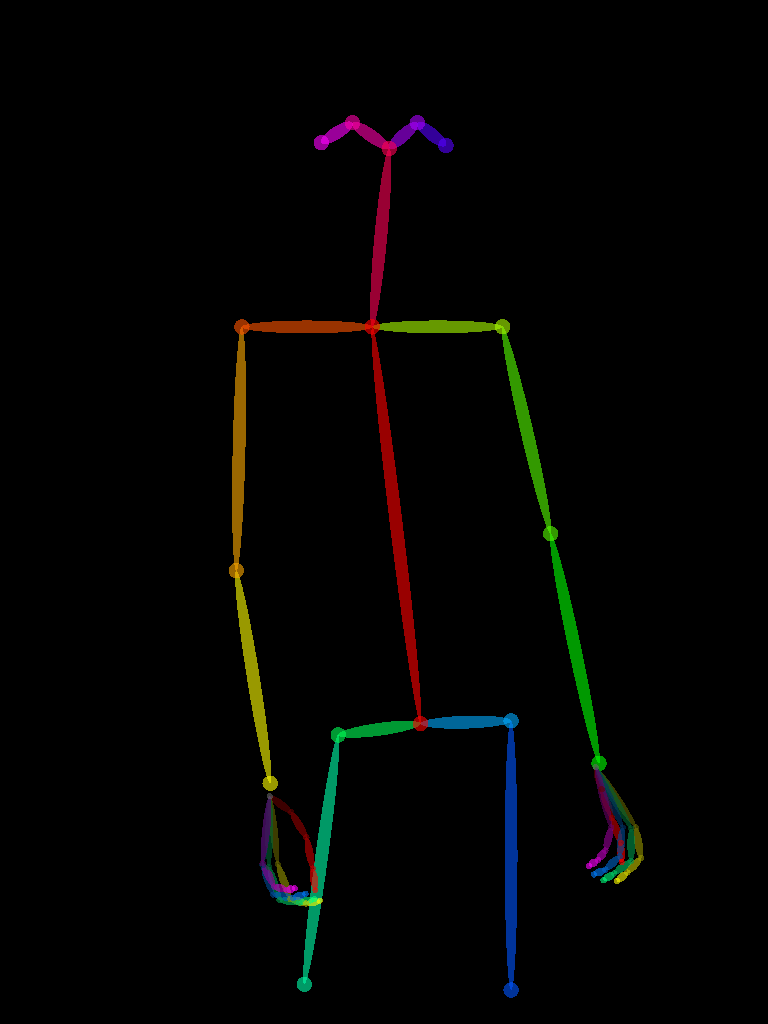
\includegraphics[width=0.55\linewidth]{images/practice_openpose.png}
    \caption{Пример изображения из \texttt{openpose\_img}}
    \label{fig:practice_openpose}
\end{figure}

\include{practice/launch}
\subsection{Запуск проектов}
\subsubsection{Технические характеристики}
Исполнение существующих проектов осуществлялось с помощью файла \texttt{inference.py}, который доступен в каждом из рассматриваемых проектов. В контексте машинного обучения, \texttt{inference} означает оценку результативности модели на похожих данных. В этом состоянии модель не обучается и не тестируется, а лишь выдаёт результаты, под которые ранее происходило обучение.

В силу нехватки вычислительных ресурсов, а также высоких системных требований у диффузионных моделей, по мере проведения экспериментов всё более актуальных \texttt{SOTA} (state of the art) моделей, требуется больше вычислительных ресурсов. Данное замечание является серьёзным недостатком решений \texttt{LaDI"=VITON} и \texttt{PromptDresser}. Таблицу с характеристиками вычислительных машин для каждого из рассматриваемых решений можно увидеть в таблице \ref{tab:tech_models}.


\begin{table}[H]
\small
\begin{tabularx}{\linewidth}{lXXX}
      & PASTA-GAN++ & LaDI-VITON & PromptDresser \\
\hline
GPU  & GeForce GTX 1060 3GB & GeForce RTX 2060 8GB & GeForce GTX 1070 8GB \\
CPU  & Intel Core i5-6400   & AMD Ryzen 7 2700 AM4     & Intel Core i5-8400 \\
RAM  & 16GB DDR4     & 16GB DDR4       & 32GB DDR4 \\
\end{tabularx}
\caption{Технические характеристики вычислительных машин для каждой из моделей. Несмотря на разницу в вычислительных ресурсах, \texttt{PromptDresser} требует значительно больше времени для генерации изображений.}
\label{tab:tech_models}
\end{table}


В рамках оценивания результатов использовались такие метрики, как \texttt{LPIPS} и \texttt{FID}. Они являются наиболее предпочтительными на фоне \texttt{MSE} и подобных функций, поскольку позволяют сравнивать изображения на основе не просто пикселей, а более глубоких признаков, таких как яркость и цветной состав.

\subsubsection{FID}
\texttt{FID} (Fréchet Inception Distance) представляет собой метрику, которая оценивает сходство между двумя наборами изображений путем сравнения их статистических характеристик в пространстве признаков. Таким образом, \texttt{FID} сравнивает распределение сгенерированных изображений с распределением изображений из исходного набора данных. Данная метрика вычисляется с помощью формулы, которая представляет собой 2"=Wasserstein расстояние между двумя многомерными гауссовскими распределениями \cite{fid}:
\begin{gather}
FID(\mu_r, \Sigma_r, \mu_g, \Sigma_g) = ||\mu_r - \mu_g||_2^2 + Tr(\Sigma_r + \Sigma_g - 2(\Sigma_r \Sigma_g)^{\frac{1}{2}}),
\end{gather}
где $(\mu_r, \Sigma_r)$ есть выборочное среднее и ковариационная матрица реальных признаков, $(\mu_g, \Sigma_g)$ "--- выборочное среднее и ковариационная матрица сгенерированных признаков, $Tr(\cdot)$ представляет собой операцию взятия следа от матрицы.

Ключевым предположением \texttt{FID} является то, что распределения признаков как реальных, так и сгенерированных изображений могут быть аппроксимированы многомерными нормальными распределениями . Первое слагаемое в формуле $||\mu_r - \mu_g||_2^2$ измеряет квадрат евклидова расстояния между средними двух распределений . Второе слагаемое $Tr(\Sigma_r + \Sigma_g - 2(\Sigma_r \Sigma_g)^{1/2})$ учитывает различия в ковариационных структурах, что позволяет оценить разнообразие изображений в рассматриваемых наборах.

В рамках анализа, для вычисления \texttt{FID} были использованы библиотеки \texttt{torchvision}, \texttt{scipy} и \texttt{numpy} для исполнения операций из линейной алгебры, \texttt{PIL} для считывания изображений, \texttt{matplotlib} для визуализации результатов. Код программы, вычисляющей \texttt{FID}, можно увидеть в приложении \ref{app:fid}. Результаты вычисления метрики можно увидеть на рисунке \ref{fig:fid_results}. \cite{fid}.

\begin{figure}[H]
    \centering
    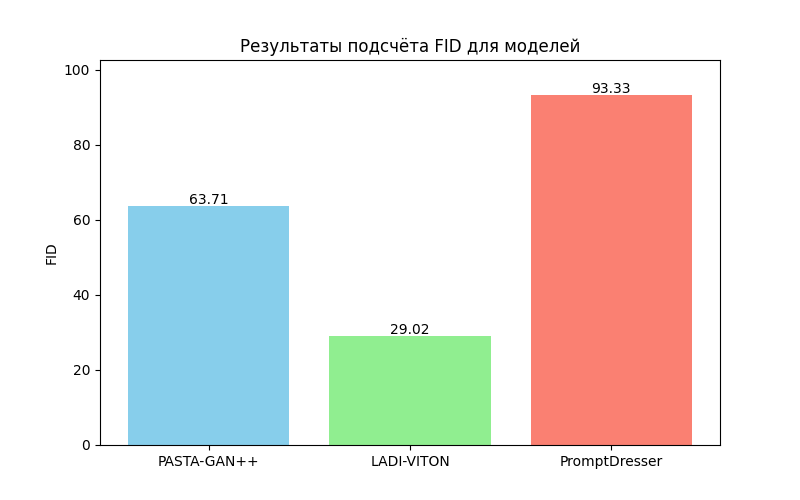
\includegraphics[width=0.85\linewidth]{images/fid_results.png}
    \caption{Результаты вычисления \texttt{FID}.}
    \label{fig:fid_results} 
\end{figure}

\subsubsection{LPIPS}
\texttt{LPIPS} (\texttt{Learned Perceptual Image Patch Similarity}) является оценкой цветового состава, текстуры и стиля. В основе метрики лежит использование предобученных сверточных нейронных сетей (например, \texttt{AlexNet}), которые извлекают из изображений карты признаков (feature maps) на различных уровнях абстракции. Для двух сравниваемых изображений вычисляются активации определённых слоёв сети, после чего производится их нормализация по канальному измерению.

Затем для каждой пары соответствующих карт признаков вычисляется евклидово расстояние, взвешенное специальными обучаемыми коэффициентами для каждого слоя. Итоговое значение \texttt{LPIPS} представляет собой сумму этих расстояний, усреднённую по всем слоям и пространственным координатам. Формула для рассчёта расстояния:
\begin{gather}
    d_l(x, y) = \frac{1}{H_lW_l}\sum_{h, w}||w_l \odot (\hat{F}(x)_{hw} - \hat{F}(y)_{hw}||_2^2,
\end{gather}
где $w_l$ "--- веса для слоя $l$.

Таким образом, формула \texttt{LPIPS} выглядит следующим образом:
\begin{gather}
    LPIPS(x, y) = \sum_{l \in L}d_l(x, y)
\end{gather}

Методы нормализации, представленные в виде $\hat{F}(\cdot)$, гарантируют минимизацию влияния масштаба каждого канала из карты признаков. Низкие значения \texttt{LPIPS} соответствуют высокой степени визуального сходства, а большие значения указывают на значительные различия между изображениями. Это делает \texttt{LPIPS} предпочтительной метрикой для оценки качества изображений, полученных с помощью генеративных моделей, поскольку она лучше отражает субъективное качество, чем классические метрики.

\begin{figure}[H]
    \centering
    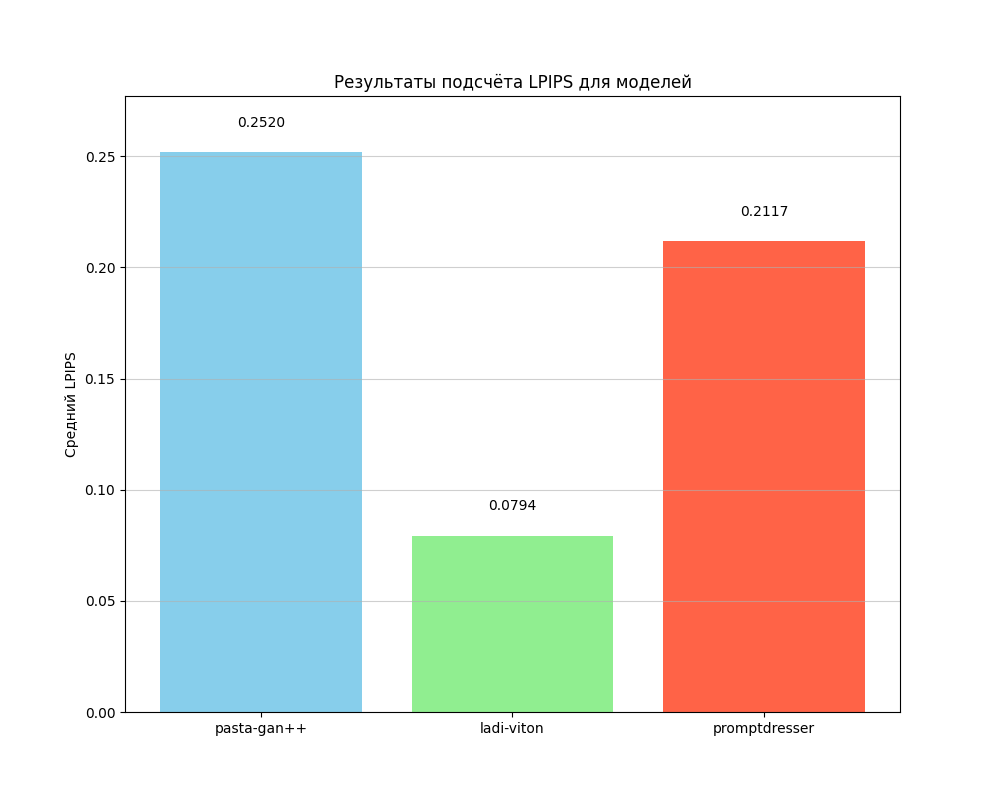
\includegraphics[width=0.9\linewidth]{images/lpips_results.png}
    \caption{Результаты вычисления \texttt{LPIPS}.}
    \label{fig:lpips_results} 
\end{figure}

Реализация метрики осуществлялась с помощью \texttt{PyTorch}, \texttt{numpy} для работы с массивами данных, \texttt{matplotlib} для визуализации результатов, а также с помощью вспомогательной библиотеки \texttt{lpips}. Код вычисления метрики можно увидеть в приложении \ref{app:lpips}, результаты можно увидеть на изображени \ref{fig:lpips_results} \cite{lpips}.

\subsection{Анализ результатов}
Согласно полученным экспериментальным данным, диффузионная модель \texttt{LaDI"=VITON} продемонстрировала превосходящие результаты по сравнению с генеративно"=состязательной архитектурой \texttt{PASTA"=GAN++} и текстово"=управляемой системой \texttt{PromptDresser}. Успех данного подхода обусловлен фундаментальными преимуществами диффузионных моделей перед альтернативными архитектурами. Диффузионные модели осуществляют генерацию изображений посредством итеративного процесса удаления шума, что позволяет им более точно моделировать сложные распределения данных и генерировать фотореалистичные изображения. Несмотря на превосходящие результаты, диффузионные модели характеризуются значительно более высокими вычислительными требованиями по сравнению с альтернативными подходами.

Однако каждый из подходов имеет свои особенности, преимущества и ограничения в контексте их архитектурных решений.
\texttt{PASTA"=GAN++} продемонстрировала худшие результаты в сравнении с диффузионной моделью, однако и требование к вычислительной машине соответственно тоже значительно ниже. Данные результаты объясняются фундаментальными проблемами, присущими \texttt{GAN}"=архитектурам, таким как нестабильность в обучении при доминации одной сети над другой. \texttt{PromptDresser}, реализующий подход генерации одежды на основе текстовых запросов, столкнулся проблемой в сложности точного перевода текстовых описаний в визуальные характеристики одежды, особенно для сложных атрибутов, таких как текстура, стиль посадки и детали кроя.


 \newpage
\conclusion
В ходе выполнения курсовой работы были подробно рассмотрены основные понятия генеративного компьютерного зрения, что позволило сформировать необходимые знания для всестороннего анализа рассматриваемой задачи. Помимо этого, были выбраны и рассмотрены разные подходы к решению задачи виртуальной примерочной. В теоретической части рассмотрены принципы работы основных генеративных моделей, таких как \texttt{GAN} и диффузионных нейронных сетей. Особое внимание было уделено каждому конкретному решению (\texttt{PASTA"=GAN++}, \texttt{LaDI"=VITON}, \texttt{PromptDresser}), включая применяемые в них модули, а также выбранные функции потерь.

В практической части была определена структура требуемого набора данных, а также с помощью вспомогательных алгоритмов и ручной разметки был составлен собственный набор данных, который применялся для тестирования рассматриваемых решений. В ходе практики удалось установить, какое решение является наиболее предпочтительным в рамках задачи виртуальной примерочной в зависимости от требуемых целей и условий. 

Для оценки качества результатов каждого из решений, были выбраны метрики \texttt{FID} и \texttt{LPIPS}. Они позволяют определить сходство между изображениями на более глубоком уровне, оперируя более сложными признаками и характеристиками изображений в целом. Такой подход позволяет более объективно оценить качество работы каждого из рассматриваемых решений.

Экспериментальные результаты подтверждают, что диффузионные модели, представленные \texttt{LADI"=VITON}, обеспечивают наилучшее качество генерации в задачах виртуальной примерки одежды за счет своей способности к точному моделированию сложных распределений данных. Однако это преимущество достигается ценой значительного увеличения вычислительных требований, что может ограничивать их практическое применение в условиях ограниченных ресурсов.

Несмотря на достигнутые результаты, в ходе работы были выявлены трудности, связанные с острым дефицитом вычислительных мощностей, разнообразием функций потерь и спецификой каждой позы, что затрудняло их сравнение. Развитие данной работы может быть направлено на более глубокую практическую часть, включая преодоление ограничений вычислительных ресурсов, введение дополнительных метрик, а также анализ других генеративных моделей.

% Раздел "Обозначения и сокращения". Может отсутствовать в работе
% \abbreviations
% \begin{description}
%     \item ... "--- ...
%     \item ... "--- ...
% \end{description}

% Раздел "Определения". Может отсутствовать в работе
% \definitions

% Раздел "Определения, обозначения и сокращения". Может отсутствовать в работе.
% Если присутствует, то заменяет собой разделы "Обозначения и сокращения" и
% "Определения"
% \defabbr


% После введения — серии \section, \subsection и т.д.

% Библиографический список, составленный вручную, без использования BibTeX
%
% \begin{thebibliography}{99}
%   \bibitem{Ione} Источник 1.
%   \bibitem{Itwo} Источник 2
% \end{thebibliography}

% Отобразить все источники. Даже те, на которые нет ссылок.
% \nocite{*}

% Меняем inputencoding на лету, чтобы работать с библиографией в кодировке
% `cp1251', в то время как остальной документ находится в кодировке `utf8'
% Credit: Никита Рыданов
\newpage
\bibliographystyle{ugost2003}
\bibliography{thesis}
% При использовании biblatex вместо bibtex
% \printbibliography

\appendix
% Окончание основного документа и начало приложений Каждая последующая секция
% документа будет являться приложением
\section{Вычисление \texttt{FID}}\label{app:fid}
Требуемое содержимое корня:
\begin{verbatim}
    computing_metrics/
    |--GAN/
    |--LADI/
    |--PROMPT/
    |--image/
    |--compute_fid.py
\end{verbatim}
Содержимое файла \texttt{compute\_fid.py}:
\begin{minted}[fontsize=\small, breaklines=true, style=bw, linenos]{python}
import os
import numpy as np
from PIL import Image
import torch
import torchvision.transforms as transforms
from torchvision.models import inception_v3
from scipy import linalg
import matplotlib.pyplot as plt

def load_and_preprocess_matched(source_folder: str, target_folder: str):
    transform = transforms.Compose([
        transforms.Resize((299, 299)),
        transforms.ToTensor(),
        transforms.Normalize(mean=[0.485, 0.456, 0.406],
                             std=[0.229, 0.224, 0.225])
    ])
    # Словари: имя_без_расширения -> имя_файла
    source_files = {os.path.splitext(f)[0]: f for f in os.listdir(source_folder) if f.lower().endswith(('.jpg', '.png'))}
    target_files = {os.path.splitext(f)[0]: f for f in os.listdir(target_folder) if f.lower().endswith(('.jpg', '.png'))}
    # Пересечение по имени
    common_keys = sorted(set(source_files.keys()) & set(target_files.keys()))
    src_imgs, tgt_imgs = [], []
    for key in common_keys:
        src_img = Image.open(os.path.join(source_folder, source_files[key])).convert('RGB')
        tgt_img = Image.open(os.path.join(target_folder, target_files[key])).convert('RGB')
        src_imgs.append(transform(src_img))
        tgt_imgs.append(transform(tgt_img))

    if src_imgs and tgt_imgs:
        return torch.stack(src_imgs), torch.stack(tgt_imgs)
    else:
        return torch.tensor([]), torch.tensor([])

def extract_feats(tensor, model, device):
    model.eval()
    feats = []
    with torch.no_grad():
        for i in range(0, len(tensor), 32):
            batch = tensor[i:i+32].to(device)
            feats.append(model(batch).cpu().numpy())
    return np.vstack(feats)

def stats(features):
    mu = np.mean(features, axis=0)
    sigma = np.cov(features, rowvar=False)
    return mu, sigma

def fid_score(mu1, sigma1, mu2, sigma2):
    diff = mu1 - mu2
    covmean = linalg.sqrtm(sigma1.dot(sigma2))
    covmean = covmean.real
    return diff.dot(diff) + np.trace(sigma1 + sigma2 - 2 * covmean)

# Вычисление FID
def get_fid(src_imgs, tgt_imgs):
    if src_imgs.nelement() == 0 or tgt_imgs.nelement() == 0:
        return None
    feats_src = extract_feats(src_imgs, model, device)
    feats_tgt = extract_feats(tgt_imgs, model, device)
    mu_s, sig_s = stats(feats_src)
    mu_t, sig_t = stats(feats_tgt)
    return fid_score(mu_s, sig_s, mu_t, sig_t)

# Пути к папкам
source = "image/"
gan = "GAN/"
ladi = "LADI/"
prompt = "PROMPT/"

device = torch.device('cuda' if torch.cuda.is_available() else 'cpu')
model = inception_v3(pretrained=True)
model.fc = torch.nn.Identity()
model.to(device)

#Загрузка файлов
src_gan_src, src_gan_tgt = load_and_preprocess_matched(source, gan)
src_ladi_src, src_ladi_tgt = load_and_preprocess_matched(source, ladi)
src_prm_src, src_prm_tgt = load_and_preprocess_matched(source, prompt)



fid_gan = get_fid(src_gan_src, src_gan_tgt)
fid_ladi = get_fid(src_ladi_src, src_ladi_tgt)
fid_prm = get_fid(src_prm_src, src_prm_tgt)

#Вывод результатов
models = []
values = []
if fid_gan is not None:
    models.append("PASTA-GAN++")
    values.append(fid_gan)
if fid_ladi is not None:
    models.append("LADI-VITON")
    values.append(fid_ladi)
if fid_prm is not None:
    models.append("PromptDresser")
    values.append(fid_prm)

for m, v in zip(models, values):
    print(f"FID для {m}: {v:.2f}")

#Отображение графика, сохранение
plt.figure(figsize=(8, 5))
bars = plt.bar(models, values, color=['skyblue', 'lightgreen', 'salmon'][:len(values)])
plt.ylabel("FID")
plt.title("Результаты подсчёта FID для моделей")

for bar, value in zip(bars, values):
    plt.text(bar.get_x() + bar.get_width()/2, value + 0.5, f"{value:.2f}", ha='center')

plt.ylim(0, max(values)*1.1)
plt.show()
plt.savefig('fid_results.png')
\end{minted}
\section{Вычисление \texttt{LPIPS}}\label{app:lpips}
Требуемое содержимое корня:
\begin{verbatim}
    computing_metrics/
    |--GAN/
    |--LADI/
    |--PROMPT/
    |--image/
    |--compute_lpips.py
\end{verbatim}
Содержимое файла \texttt{compute\_lpips.py}:
\begin{minted}[fontsize=\small, breaklines=true, style=bw, linenos]{python}
import lpips
import torch
import matplotlib.pyplot as plt
import numpy as np
from PIL import Image
import os

device = 'cuda' if torch.cuda.is_available() else 'cpu'

# Инициализация LPIPS
loss_fn = lpips.LPIPS(net='alex').to(device)

def load_image(path):
    img = Image.open(path).convert('RGB')
    img = img.resize((256, 256))  
    img_tensor = torch.from_numpy(np.array(img)).permute(2,0,1).float() / 255.0
    img_tensor = img_tensor.unsqueeze(0) * 2 - 1 
    return img_tensor

def calculate_lpips(source_folder, result_folder, source_files, result_files):
    scores = []
    
    for src, res in zip(source_files, result_files):
        if src.split('.')[0] == res.split('.')[0]:
            src_path = os.path.join(source_folder, src)
            res_path = os.path.join(result_folder, res)

            img1 = load_image(src_path).to(device)
            img2 = load_image(res_path).to(device)

            with torch.no_grad():
                dist = loss_fn(img1, img2)
            scores.append(dist.item())
    return scores

#Обозначение необходимой информации: папки, список файлов, словари для хранения значений метрик
gan_folder = "GAN/"
ladi_folder = "LADI/"
prompt_folder = "PROMPT/"
source_folder = "image/"

ladi_files = [f for f in os.listdir(ladi_folder) if f.lower().endswith(".jpg")]
prompt_files = [f for f in os.listdir(prompt_folder) if f.lower().endswith(".jpg")]
source_files = [f for f in os.listdir(source_folder) if f.lower().endswith(".jpg")]
gan_files = [f for f in os.listdir(gan_folder) if f.lower().endswith(".png")]

#Подсчёт метрик для каждой модели
gan_scores = calculate_lpips(source_folder, gan_folder, source_files, gan_files)
ladi_scores = calculate_lpips(source_folder, ladi_folder, source_files, ladi_files)
prompt_scores = calculate_lpips(source_folder, prompt_folder, source_files, prompt_files)

#Вывод среднего значения для каждой модели
mean_score = [np.mean(gan_scores), np.mean(ladi_scores), np.mean(prompt_scores)]
models = ['pasta-gan++', 'ladi-viton', 'promptdresser']

for model, score in zip(models, mean_score):
    print(f"Средний LPIPS для {model}: {score:.4f}")

#Настройка графика (BarPlot)
plt.figure(figsize=(10, 8))
bars = plt.bar(models, mean_score, color=['skyblue', 'lightgreen', 'tomato'])
plt.ylim(0, max(mean_score)*1.1)

plt.ylabel('Средний LPIPS')
plt.title('Результаты подсчёта LPIPS для моделей')
plt.grid(axis='y', alpha=.6)

#Добавление значений на график
for bar in bars:
    yval = bar.get_height()
    plt.text(bar.get_x() + bar.get_width()/2, yval + 0.01, f"{yval:.4f}", ha='center', va='bottom')

#Отображение графика, его сохранение
plt.show()
plt.savefig("lpips_results.png")
\end{minted}

\end{document}
